\documentclass{report}
\usepackage[spanish]{babel}
\usepackage[utf8]{inputenc}
\usepackage{graphicx, longtable, float, titlesec, hyperref, xcolor}

\hypersetup{
    hidelinks = true
}

\titleformat{\chapter}[display]
  {\normalfont\bfseries}{}{0pt}{\Huge}

\begin{document}
    \begin{titlepage}
        \centering
        
\includegraphics[width=0.6\textwidth]{./img/miscelanio/logo.jpg}\\
        \vspace{1cm}
        \LARGE Sistemas de Gestión de Seguridad de Sistemas de Información\\
        \vspace{0.5cm}
        \Large Ingeniería Informática de Gestión y Sistemas de Información\\
        \vspace{3cm}
        \Huge Sistema Web\\
        \vspace{2.5cm}
        \Large Autores:\\
        \vspace{0.2cm}
        \large Xabier Gabiña\\
        \large Ainhize Martinez\\
        \large Marcos Martín\\
        \vfill
        \today
    \end{titlepage}
    \tableofcontents
    \chapter{Introducción}
        La finalidad de esta etapa del proyecto es garantizar la seguridad y robustez de la página web desarrollada en la fase inicial del proyecto. Con el propósito de lograr este objetivo, se recurrirá a la aplicación de diversas herramientas y técnicas que han sido abordadas y exploradas a lo largo del curso. El enfoque principal de esta fase se centra en identificar y abordar posibles vulnerabilidades y debilidades de seguridad en el sistema, a fin de implementar medidas correctivas y fortalecer la integridad de la plataforma web.\\
        
        Este proceso implica la utilización de herramientas especializadas, como ZAP, SQLMap, Nmap y Metasploit, que permiten evaluar y poner a prueba la infraestructura de seguridad de la página web. A través de su empleo, se llevará a cabo un exhaustivo análisis que permitirá descubrir posibles fallos o vulnerabilidades que puedan ser aprovechadas por actores maliciosos, poniendo en riesgo la integridad de los datos y la privacidad de los usuarios.\\
        
        El objetivo último es la identificación, documentación y solución de posibles vulnerabilidades, lo que contribuirá a elevar la seguridad y confiabilidad de la página web. A medida que se avance en este proceso, se aplicarán estrategias y medidas correctivas para abordar los hallazgos identificados y se establecerán salvaguardias que minimicen el riesgo de futuros incidentes de seguridad.\\
        
        Este proyecto representa un ejercicio académico valioso que no solo demuestra la comprensión de los conceptos de seguridad informática, sino que también ofrece la oportunidad de aplicar de manera práctica las habilidades adquiridas en la detección y mitigación de riesgos en entornos web. A través de esta experiencia, se espera adquirir un conocimiento más profundo y aplicable en el campo de la seguridad informática y estén mejor preparados para enfrentar desafíos en el mundo real.\\
    \chapter{Primera auditoría}
        El objetivo principal de esta auditoría es la de encontrar los fallos de seguridad que tiene nuestro sistema web para poder solucionarlos en el sigueite capítulo de este documento.
        \section{ZAP}
            Para empezar con la primera auditoría ejecutaremos el proxy ZAP como se nos ha propuesto en clase.\\
            
            ZAP es una herramienta de seguridad de aplicaciones web de código abierto que se utiliza para encontrar automáticamente vulnerabilidades en las aplicaciones web. Está diseñado para ser accesible a usuarios con diversos niveles de experiencia y conocimientos en seguridad, y como tal es ideal para desarrolladores y probadores funcionales que son nuevos en el ámbito de la seguridad de aplicaciones web.\\
            
            En nuestro caso usamos AJAX por lo que debemos especificar al ejecutar AJAX que usa la SPIDER AJAX en ZAP.\\
            
            Al ejecutarla en nuestra página web, nos encontramos con el siguiente listado de errores y fallos de configuración:
            \begin{figure}[H]
                \centering
                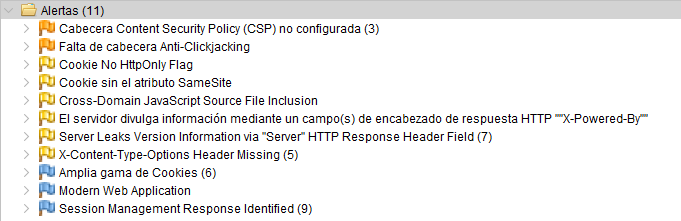
\includegraphics[width=0.8\textwidth]{./img/audit1/zap1.png}
                \caption{Listado de errores de la primera auditoría}
            \end{figure}
            Como podemos ver en la imagen, tenemos un total de 16 errores.
            Estos errores son por lo general de configuraciones tanto del servidor web como de la página web.

        \clearpage
        \section{sqlmap}
            La siguiente herramienta que usaremos será sqlmap, la cual nos permitirá encontrar fallos de seguridad en la base de datos y en los formularios que hacen uso de ella.
            \begin{figure}[H]
                \centering
                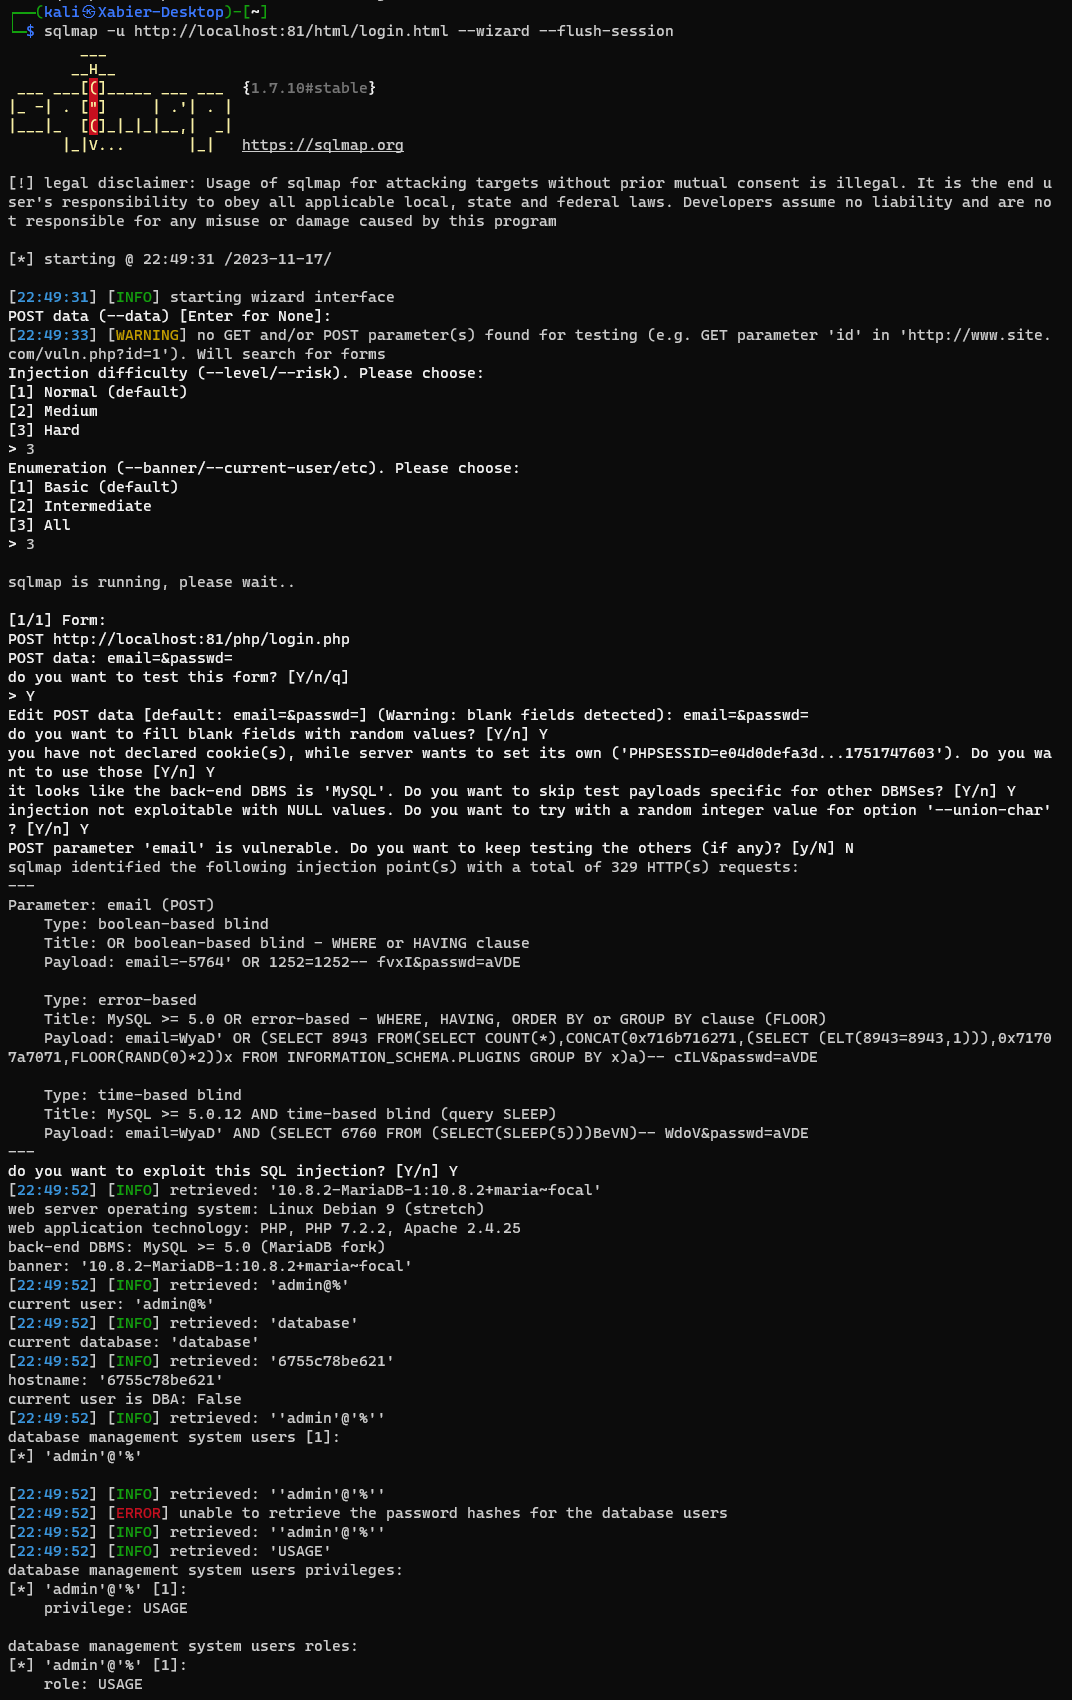
\includegraphics[width=0.80\textwidth]{./img/audit1/sqlmap1.png}
                \caption{Output de sqlmap 1}
            \end{figure}
            \begin{figure}[H]
                \centering
                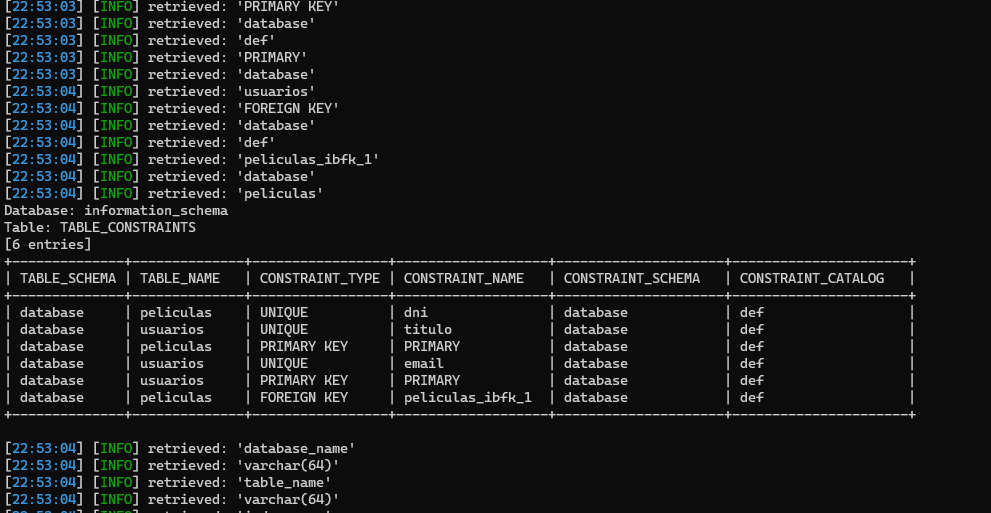
\includegraphics[width=\textwidth]{./img/audit1/sqlmap2.png}
                \caption{Output de sqlmap 2}
            \end{figure}
            \begin{figure}[H]
                \centering
                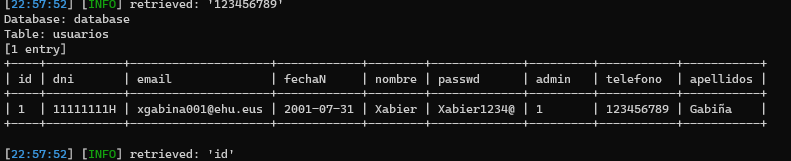
\includegraphics[width=\textwidth]{./img/audit1/sqlmap3.png}
                \caption{Output de sqlmap 3}
            \end{figure}
            \begin{figure}[H]
                \centering
                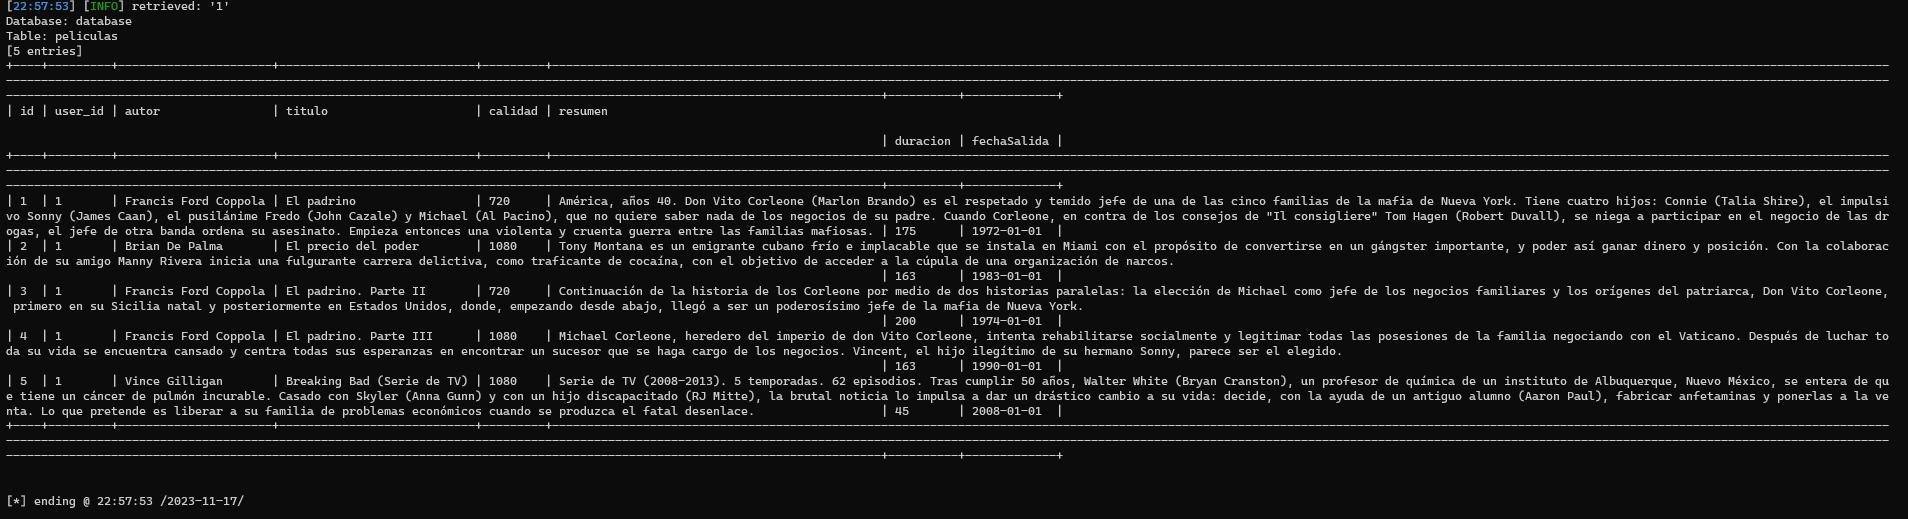
\includegraphics[width=\textwidth]{./img/audit1/sqlmap4.png}
                \caption{Output de sqlmap 4}
            \end{figure}
            Al terminar este proceso podemos ver que nos ha mostrado todo el contenido de la base de datos por pantalla además de la version del servidor, de php y de la propia base de datos.

            Además, al tener las contraseñas en texto plano cualquiera podría loguearse como un usuario y acceder a la página suplantándolo.
        \clearpage
        \section{nmap}
            La siguiente herramienta que usaremos será nmap. Nmap es utilizada para descubrir hosts y servicios en una computadora en una red, creando un mapa de la misma. Para lograr su propósito, Nmap envía paquetes de datos sin procesar a través de la red y luego analiza las respuestas.
            \begin{figure}[H]
                \centering
                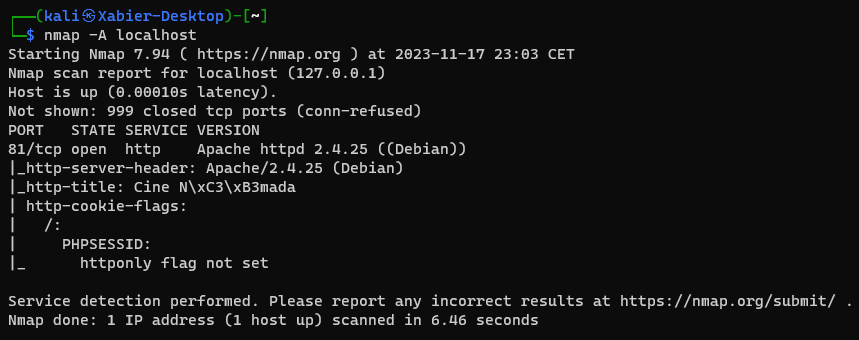
\includegraphics[width=\textwidth]{./img/audit1/nmap1.png}
                \caption{Output de nmap 1}
            \end{figure}
            Como podemos ver nmap ha detectado el servidor web y nos ha arrojado información como su puerto y su versión.
            Esto es una vulnerabilidad, ya que al saber la versión se puede hacer uso de bases de datos, como la de exploitDB, para encontrar exploits que puedan ser usados contra nuestro servidor.
        \clearpage
        \section{Metaexploit}
            En este caso, he usado la herramienta Metaexploit para comprobar si nuestro sistema web es vulnerable a algún exploit conocido.
            Metaexploit es un framework de pruebas de penetración que permite a los usuarios crear, probar y desplegar exploits contra sistemas de seguridad.
            
            Tras algunas búsquedas, se ha encontrado un exploit que mediante diccionarios de contraseñas intenta loguearse en phpMyAdmin.
            \begin{figure}[H]
                \centering
                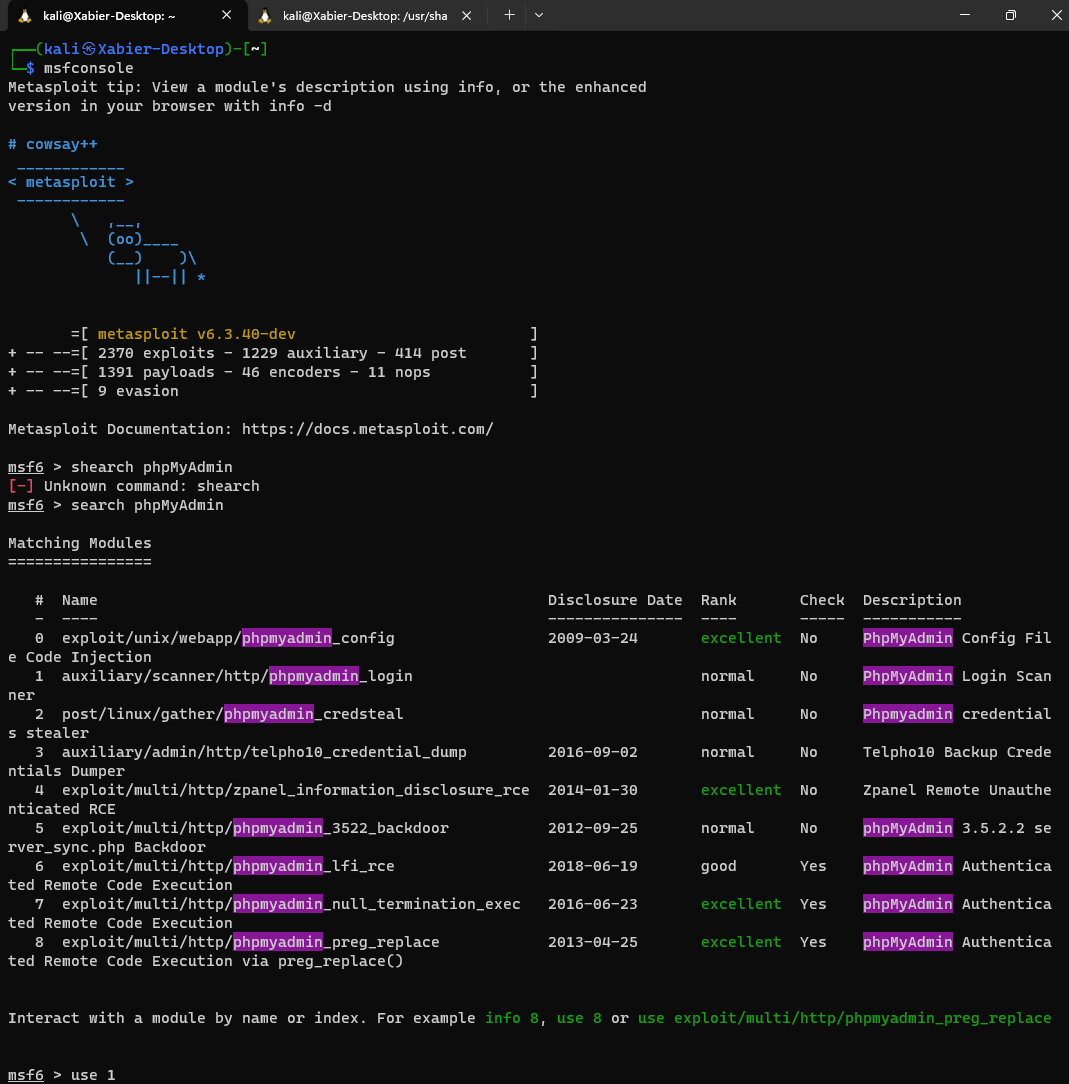
\includegraphics[width=\textwidth]{./img/audit1/msf1.png}
                \caption{Output de metasploit 1}
            \end{figure}
            \begin{figure}[H]
                \centering
                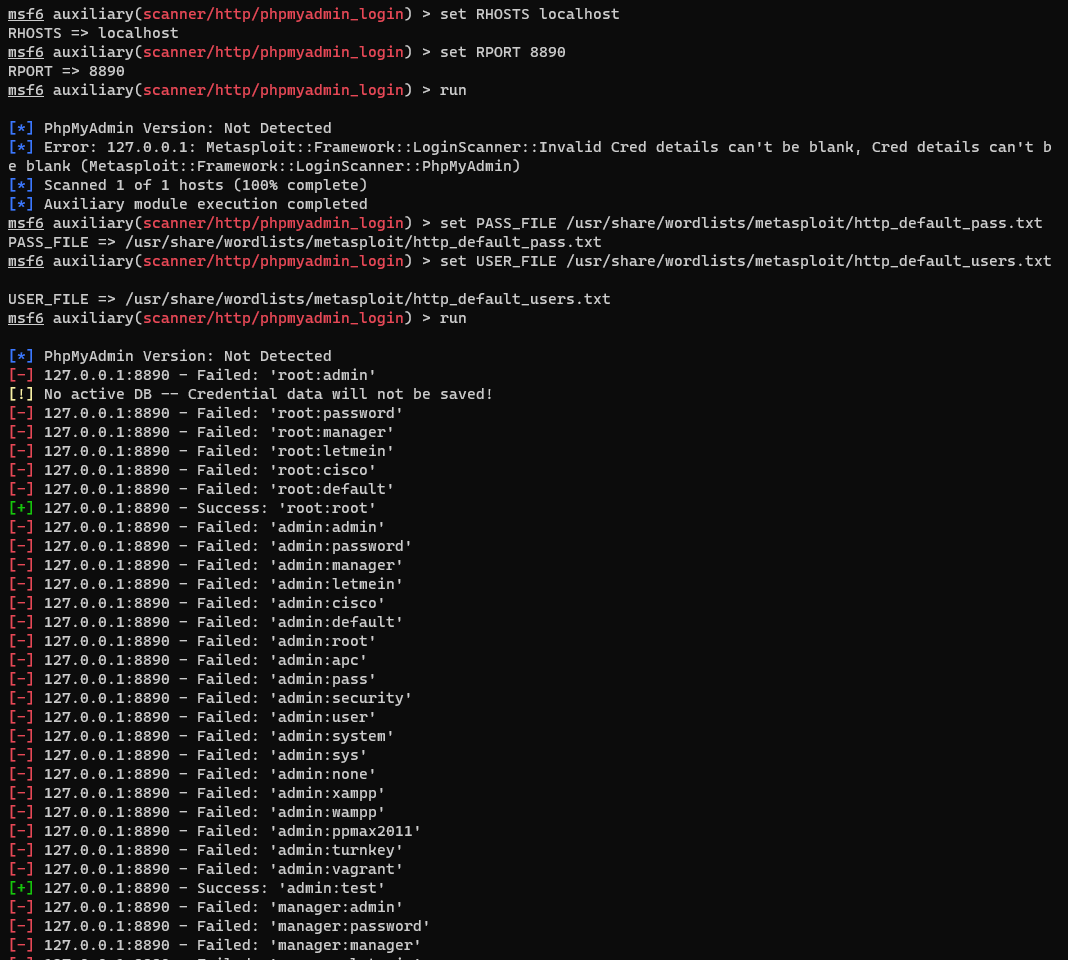
\includegraphics[width=\textwidth]{./img/audit1/msf2.png}
                \caption{Output de metasploit 2}
            \end{figure}
            Al tener una contraseña tan débil, enseguida ha encontrado las credenciales de phpMyAdmin tanto para root como para el usuario admin.
            
            Esto es una vulnerabilidad del sistema ya que, al tener acceso a phpMyAdmin, se puede acceder a la base de datos y modificarla a placer.
        \clearpage
    \chapter{Vulnerabilidades}
        \section{Rotura de control de acceso}
            La rotura de control de acceso es una vulnerabilidad que permite a un atacante acceder a recursos restringidos o privilegiados, ya sea por un error en la implementación de la autenticación y autorización o por un error en la lógica de control de acceso.
            \subsection{Acceso mediante URL}
                \subsubsection{Descripción}
                    El acceso mediante URL se refiere a la práctica de manipular los parámetros presentes en una URL con el objetivo de eludir o evadir los controles de acceso implementados en un sistema o aplicación. 
                \subsubsection{Solución}
                    Esto no es un error en nuestra página web ya que al contenido no se accede mediante redirecciones en la página web, sino que se hace mediante el uso de AJAX.
                    
                    AJAX es una técnica de programación que permite que una página web se comunique con el servidor, sin necesidad de hacer redirecciones ni recargas de la página.
                    
                    Esto hace que si alguien entra en un archivo como login.php al no cargarse mediante AJAX, tampoco se cargan los archivos necesarios para que funcione por lo que es inútil.
                \clearpage
            \subsection{Acceso a cuenta personal}
                \subsubsection{Descripción}
                    En nuestro sistema, un usuario puede modificar sus datos personales, pero también puede modificar los datos de otros usuarios. 
                    Esto es un fallo de rotura de control de acceso ya que un usuario no debería poder modificar los datos de otro usuario.
                \subsubsection{PoC}
                    Pongamos en el ejemplo que tenemos dos usuarios, Admin y Xabier con sus repectivas IDs.
                    \begin{figure}[H]
                        \centering
                        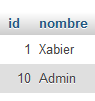
\includegraphics[width=0.2\textwidth]{./img/vulnerabilidades/3.1/1.1.png}
                        \caption{Datos de Usuarios}
                    \end{figure}
                    Si desde inspeccionar elementos hacemos click sobre el botón 'Perfil', este nos mostrará el link el cual se ve así:
                    \begin{figure}[H]
                        \centering
                        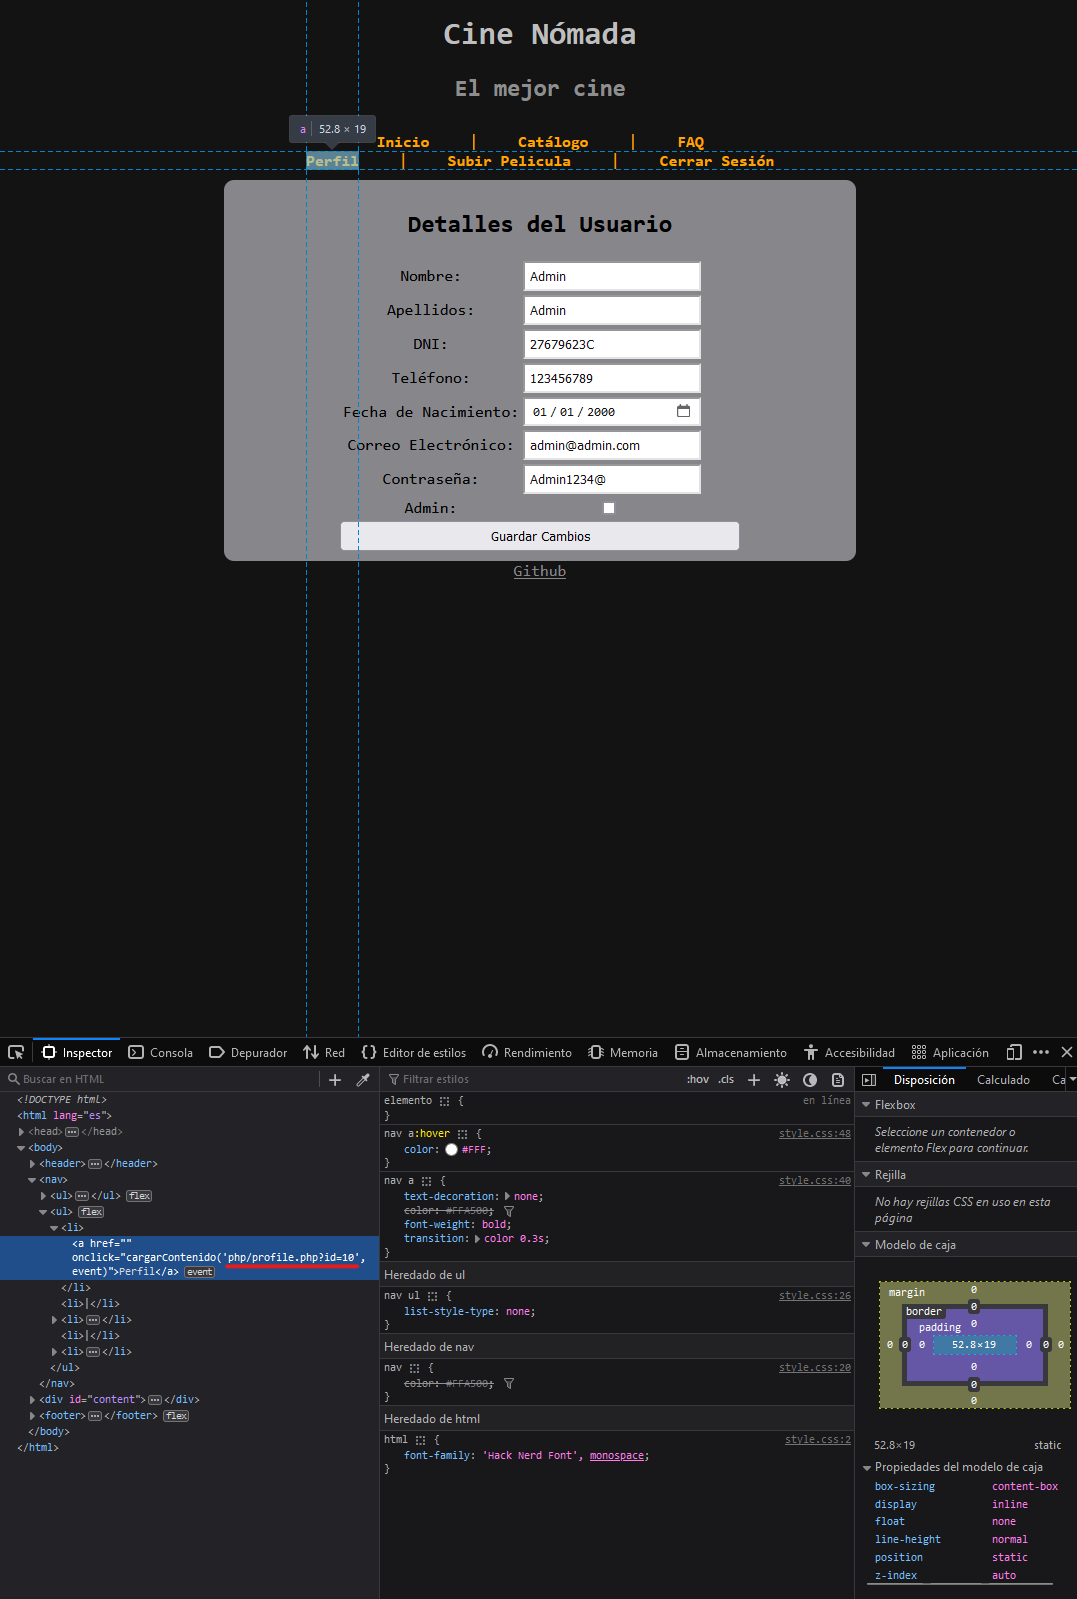
\includegraphics[width=0.8\textwidth]{./img/vulnerabilidades/3.1/1.2.png}
                        \caption{Perfil de Admin}
                    \end{figure}
                    Si alteramos el valor de '?id=X' por, en este caso, la id de Xabier (La ID 1) podemos acceder a sus datos.
                    \begin{figure}[H]
                        \centering
                        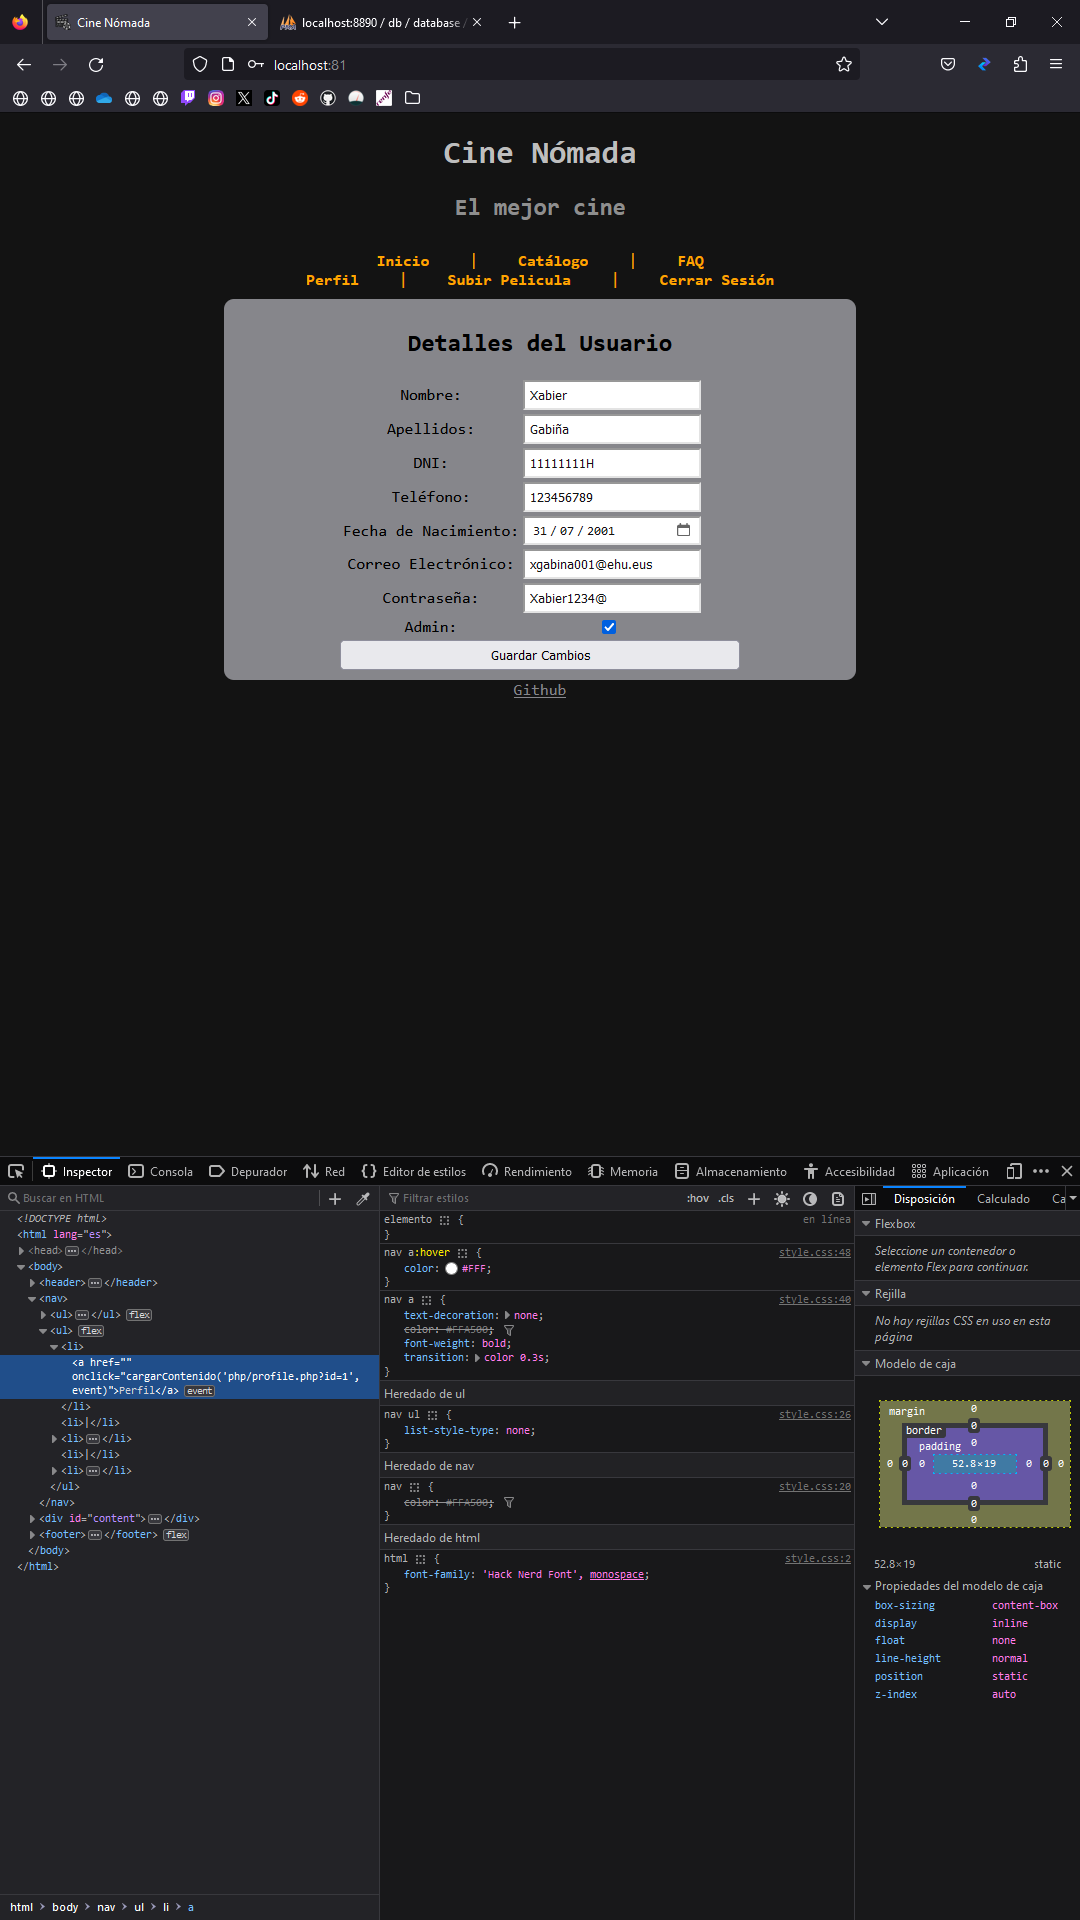
\includegraphics[width=\textwidth]{./img/vulnerabilidades/3.1/1.3.png}
                        \caption{Perfil de Xabier}
                    \end{figure}
                \subsubsection{Solución}
                    Para solucionar este problema, hemos añadido una comprobación en el código que verifica si el usuario que está intentando modificar los datos es el mismo que el usuario que está logueado en el sistema.
                    \begin{figure}[H]
                        \centering
                        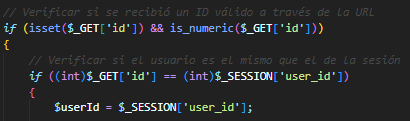
\includegraphics[width=\textwidth]{./img/vulnerabilidades/3.1/1.4.png}
                        \caption{Comprobación de usuario}
                    \end{figure}
                    Este mismo error también ha sido corregido en el catálogo.
            \clearpage       
        \section{Fallos criptográficos}
            Los "fallos criptográficos" se refieren a debilidades o errores en el diseño, implementación o uso de algoritmos criptográficos que comprometen la seguridad de la información protegida mediante técnicas de cifrado y protección.
            \subsection{Cifrado de extremo a extremo}
                \subsubsection{Descripción}
                    El cifrado de extremo a extremo es un método de seguridad informática en el que la información se cifra en el punto de origen y solo se descifra en el punto de destino. Esto significa que los datos están protegidos durante su transmisión y solo son legibles para la parte destinataria que posee la clave de descifrado correspondiente.
                \subsubsection{Solución}
                    Para solucionar este problema, configuraremos nuestro servidor para que cifre y rediriga todo el tráfico a HTTPS.
                    Creamos un certificado SSL autofirmado dentro del Dockerfile.
                    Creamos una regla para redirigir el tráfico entrante del puerto 80 al puerto 443.
                    \begin{figure}[H]
                        \centering
                        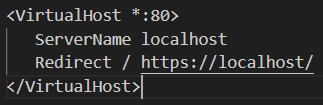
\includegraphics[width=\textwidth]{./img/vulnerabilidades/3.2/1.1.png}
                        \caption{Redirección de tráfico}
                    \end{figure}
                    
                    También debemos decir al puerto 443 que use el certificado SSL que hemos creado.
                    \begin{figure}[H]
                        \centering
                        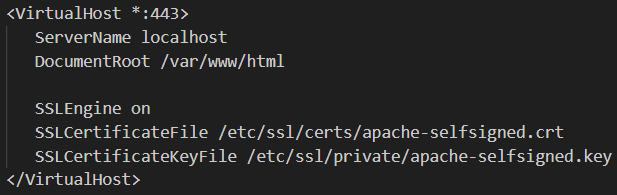
\includegraphics[width=\textwidth]{./img/vulnerabilidades/3.2/1.2.png}
                        \caption{Certificado SSL}
                    \end{figure}
            \clearpage
            \subsection{Almacenamiento de contraseñas}
                \subsubsection{Descripción}
                    En nuestro sistema, no se almacenan las contraseñas de los usuarios de forma segura, lo que permite que un atacante pueda obtener las contraseñas de los usuarios.
                \subsubsection{PoC}
                    Si un atacante consigue acceso a la base de datos, podría obtener las contraseñas de los usuarios en texto plano.
                    \begin{figure}[H]
                        \centering
                        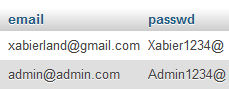
\includegraphics[width=\textwidth]{./img/vulnerabilidades/3.2/2.1.png}
                        \caption{Contraseñas en texto plano}
                    \end{figure}
                \subsubsection{Solución}
                    Para solucionar este problema de la mejor forma posible, debemos tener tres puntos bien definidos:
                    \begin{enumerate}
                        \item Cofigurar el factor de costo apropiado
                        \begin{itemize}
                            \item El factor de costo (work factor) en bcrypt determina el número de iteraciones utilizadas en el cálculo del hash. Un valor mayor implica una contraseña más segura, pero también requiere más tiempo para calcular el hash. Un valor razonable es 12 o más, dependiendo del hardware y las necesidades de rendimiento.
                        \end{itemize}
                        \item Usar un algoritmo de cifrado seguro.
                        \begin{itemize}
                            \item En nuestro caso, usaremos BCrypt. CRYPT\_BLOWFISH se usa para crear el hash. Producirá un hash estándar compatible con crypt() utilizando el identificador \texttt{"\$2y\$"}. El resultado siempre será un string de 60 carácteres, o false en caso de error.
                        \end{itemize}
                        \item Generar un semilla aleatoria para cada usuario.
                        \begin{itemize}
                            \item BCrypt ya gestiona las semillas de forma automática y en el manual de PHP no recomiendan su uso de otra manera. Mas información en: \url{https://www.php.net/manual/es/function.password-hash.php}
                        \end{itemize}
                    \end{enumerate}
                    \begin{figure}[H]
                        \centering
                        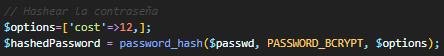
\includegraphics[width=\textwidth]{./img/vulnerabilidades/3.2/2.2.png}
                        \caption{Contraseñas encriptadas}
                    \end{figure}
            \clearpage
            \subsection{Configuración errónea de las Cookies}
                \subsubsection{Descripción}
                    La configuración errónea de las cookies se refiere a la práctica de establecer parámetros o atributos de las cookies de manera inadecuada, lo que puede tener consecuencias negativas en términos de seguridad, privacidad y funcionalidad en una aplicación web.                
                \subsubsection{Solución}
                    Para solucionar este problema, hemos añadido una configuración segura a las cookies de nuestro sitio web.
                    \begin{figure}[H]
                        \centering
                        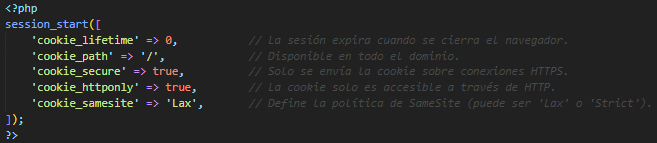
\includegraphics[width=\textwidth]{./img/vulnerabilidades/3.2/3.1.png}
                        \caption{Configuración de las cookies}
                    \end{figure}
            \clearpage
        \section{Inyección}
            En el ámbito de la seguridad informática y el desarrollo de software, el término 'inyección' se refiere a una clase de vulnerabilidades que permite a un atacante introducir y ejecutar código malicioso en una aplicación o sistema. 
            \subsection{SQL Injection}
                \subsubsection{Descripción}
                    La inyección SQL es una vulnerabilidad de seguridad informática que permite a un atacante modificar las consultas SQL que se ejecutan en una base de datos subyacente. Esto puede permitir a un atacante obtener información confidencial, alterar o eliminar datos, o incluso comprometer completamente el sistema.
                \subsubsection{Solución}
                    Para solucionar este problema, hemos modificado el código que procesa las consultas SQL para que no se puedan inyectar consultas SQL.
                    \begin{figure}[H]
                        \centering
                        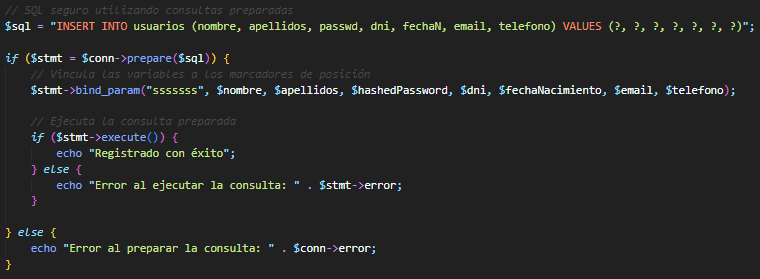
\includegraphics[width=\textwidth]{./img/vulnerabilidades/3.3/1.1.png}
                        \caption{Parametrizar consulta SQL}
                    \end{figure}
            \clearpage
            \subsection{Cross-Site Scripting (XSS)}
                \subsubsection{Descripción}
                    El Cross-Site Scripting (XSS) es una vulnerabilidad de seguridad informática que permite a un atacante inyectar código malicioso (por lo general JavaScript) en páginas web que son vistas por otros usuarios. El XSS permite a los atacantes ejecutar scripts en el navegador de un usuario, lo que puede secuestrar sesiones de usuario, desfigurar sitios web, robar información confidencial y distribuir malware.
                \subsubsection{Solución}
                    La solución a este problema se verá más adelante en la sección 3.5.5.
            \clearpage
            \subsection{Cross-Site Request Forgery}
                \subsubsection{Descripción}
                    El Cross-Site Request Forgery (CSRF) es una vulnerabilidad de seguridad informática que permite a un atacante forzar a un usuario autenticado a ejecutar acciones no deseadas en una aplicación web en la que confía. El CSRF puede utilizarse para realizar acciones como transferencias de fondos, cambios de contraseñas, compras, etc.
                \subsubsection{Solución}
                    Para solucionar este problema, hemos añadido un token CSRF a nuestro sitio web.
                    \begin{figure}[H]
                        \centering
                        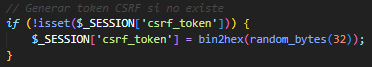
\includegraphics[width=\textwidth]{./img/vulnerabilidades/3.3/3.1.png}
                        \caption{Token CSRF}
                    \end{figure}
                    \begin{figure}[H]
                        \centering
                        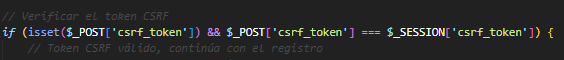
\includegraphics[width=\textwidth]{./img/vulnerabilidades/3.3/3.2.png}
                        \caption{Comprobación de token CSRF}
                    \end{figure}
            \clearpage
        \section{Diseño inseguro}
            El "diseño inseguro" se refiere a la presencia de debilidades fundamentales en el diseño de una aplicación web que pueden ser explotadas por atacantes para comprometer la seguridad.
            \subsection{Reutilización de códigos seguros}
                \subsubsection{Descripción}
                    La reutilización de código seguro se refiere a la práctica de aprovechar componentes de software previamente probados y seguros en lugar de escribir código desde cero. Esto no solo puede acelerar el desarrollo de software, sino que también puede reducir el riesgo de introducir vulnerabilidades de seguridad.
                \subsubsection{Solución}
                    En nuestro proyecto, se han implementado estas prácticas mediante la reutilización del archivo validar.js en el que se encuentran las funciones de validación de todos los formularios de nuestro sitio web.
                    \begin{figure}[H]
                        \centering
                        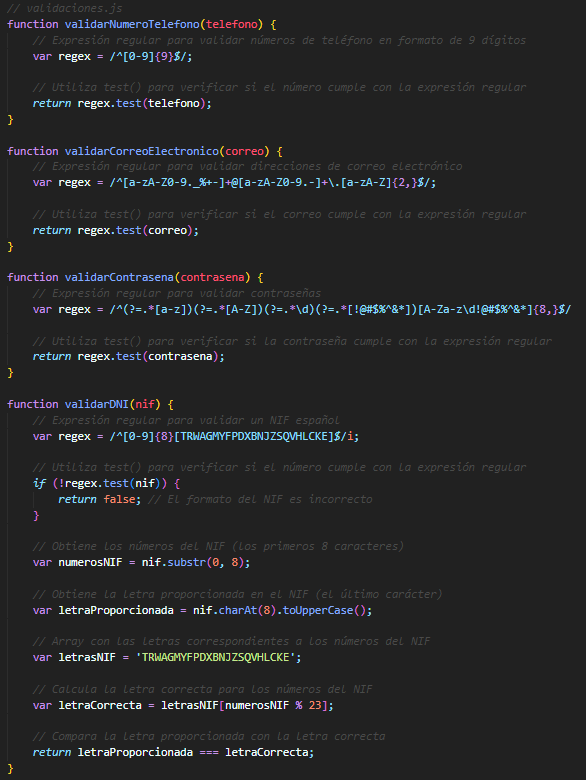
\includegraphics[width=\textwidth]{./img/vulnerabilidades/3.4/1.1.png}
                        \caption{Validación de formularios}
                    \end{figure}
            \clearpage
        \section{Configuración de seguridad insuficiente}
            La configuración de seguridad incorrecta o insuficiente se refiere a ajustes o parámetros de seguridad que no están adecuadamente configurados para proteger un sistema, aplicación, red o servicio. Puede haber varias áreas en las que la configuración de seguridad puede ser insuficiente o incorrecta, lo que podría dejar un sistema vulnerable a amenazas y ataques.
            \subsection{Despliegue seguro}
                \subsubsection{Descripción}
                    Es importante que a la hora de montar nuestro servidor web no haya archivos que puedan ser accesibles desde el exterior y que puedan contener información sensible como contraseñas. Esto a nosotros nos ocurre en el docker-compose.yml
                \subsubsection{Solución}
                    Hemos creado un .env donde se almacenan las contraseñas y el resto de información sensible y hemos añadido el archivo al .gitignore para que no se suba al repositorio.
                    Dado que esto es un trabajo, el .env será incluido para poder comprobar que funciona correctamente.
                    \begin{figure}[H]
                        \centering
                        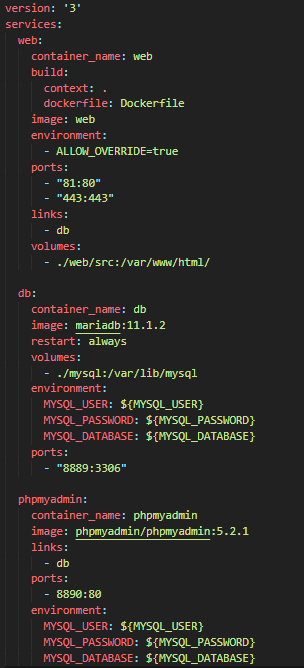
\includegraphics[width=0.7\textwidth]{./img/vulnerabilidades/3.5/1.1.png}
                        \caption{docker-compose sin información sensible}
                    \end{figure}
            \clearpage
            \subsection{Cabecera CSP}
                \subsubsection{Descripción}
                    Las cabeceras CSP son una medida de seguridad utilizada en la programación web para mitigar los riesgos asociados con ataques de Cross-Site Scripting (XSS) y otros tipos de ataques de inyección de código malicioso en páginas web.
                \subsubsection{Solución}
                    Para solucionar este problema, hemos añadido una cabecera 'Content-Security-Policy' con los siguientes valores:
                    \begin{figure}[H]
                        \centering
                        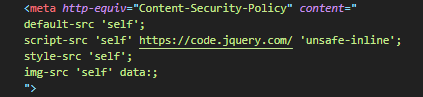
\includegraphics[width=\textwidth]{./img/vulnerabilidades/3.5/2.1.png}
                        \caption{Cabecera CSP}
                    \end{figure}
                    En este caso, nos hemos visto obligados a usar la etiqueta 'unsafe-inline' ya que, si no la usamos, no se cargan las bibliotecas de jQuery y reCAPTCHA.
                    Esto podría ser un problema con librerías inseguras pero en nuestro caso no lo es ya que las librerías que usamos son de confianza.
            \clearpage
            \subsection{Cabecera Cache-Control}
                \subsubsection{Descripción}
                    Las cabeceras 'Cache-Control' son utilizadas en las respuestas HTTP enviadas por un servidor web para controlar cómo los recursos web deben ser almacenados en la memoria caché del navegador o en servidores intermedios (como proxies) y cómo se deben comportar en términos de almacenamiento y actualización. Estas cabeceras son fundamentales para gestionar la eficiencia de la carga de páginas web, la seguridad y la privacidad.
                \subsubsection{Solución}
                    Para solucionar este problema, crearemos una cabecera 'Cache-Control' con el valor 'no-store' para que el navegador no almacene en caché la página.
                    \begin{figure}[H]
                        \centering
                        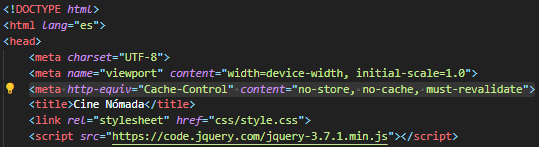
\includegraphics[width=\textwidth]{./img/vulnerabilidades/3.5/3.1.png}
                        \caption{Cabecera Cache-Control}
                    \end{figure}
            \clearpage
            \subsection{Cabecera HSTS}
                \subsubsection{Descripción}
                    Las cabeceras HSTS (HTTP Strict Transport Security) son una medida de seguridad utilizada en la programación web para garantizar que las comunicaciones entre un navegador web y un sitio web se realicen a través de una conexión segura y encriptada utilizando el protocolo HTTPS (HTTP Secure). HSTS ayuda a prevenir ataques de tipo man-in-the-middle (MitM) que podrían exponer datos sensibles o comprometer la seguridad de la comunicación.
                \subsubsection{Solución}
                    Para solucionar este problema, hemos añadido una cabecera 'Strict-Transport-Security' con los siguientes valores:
                    \begin{figure}[H]
                        \centering
                        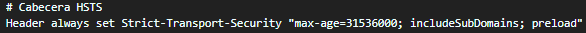
\includegraphics[width=\textwidth]{./img/vulnerabilidades/3.5/4.1.png}
                        \caption{Cabecera HSTS}
                    \end{figure}
            \clearpage
            \subsection{Cabecera X-XSS-Protection}
                \subsubsection{Descripción}
                Las cabeceras "X-XSS-Protection" son una medida de seguridad utilizada en la programación web para ayudar a prevenir ataques de tipo Cross-Site Scripting (XSS). Los ataques XSS ocurren cuando un atacante inyecta código JavaScript malicioso en una página web, que luego se ejecuta en el navegador de un usuario sin su conocimiento. Estas cabeceras se utilizan para controlar y mitigar estos ataques.
                \subsubsection{Solución}
                    Para solucionar este problema, hemos añadido una cabecera 'X-XSS-Protection' con los siguientes valores:
                    \begin{figure}[H]
                        \centering
                        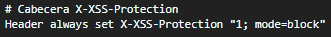
\includegraphics[width=\textwidth]{./img/vulnerabilidades/3.5/5.1.png}
                        \caption{Cabecera X-XSS-Protection}
                    \end{figure}
            \clearpage
            \subsection{Cabecera X-Content-Type-Options}
                \subsubsection{Descripción}
                Las cabeceras "X-Content-Type-Options" son una medida de seguridad utilizada en la programación web para mitigar ciertos tipos de ataques, como ataques de tipo MIME-sniffing. Estas cabeceras se utilizan para controlar cómo el navegador web interpreta y muestra el contenido de una página web.
                \subsubsection{Solución}
                    Para solucionar este problema, hemos añadido una cabecera 'X-Content-Type-Options' con los siguientes valores:
                    \begin{figure}[H]
                        \centering
                        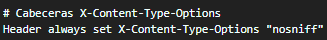
\includegraphics[width=\textwidth]{./img/vulnerabilidades/3.5/6.1.png}
                        \caption{Cabecera X-Content-Type-Options}
                    \end{figure}
            \clearpage
            \subsection{Cabecera X-Frame-Options}
                \subsubsection{Descripción}
                    Las cabeceras "X-Frame-Options" son una medida de seguridad utilizada en la programación web para controlar si una página web puede ser incrustada o mostrada dentro de un marco (frame) de otro sitio web. Estas cabeceras se utilizan para prevenir ataques de clickjacking, en los cuales un atacante puede ocultar contenido malicioso detrás de una página legítima y engañar a los usuarios para que hagan click en elementos sin su consentimiento.
                \subsubsection{Solución}
                    Para solucionar este problema, hemos añadido una cabecera 'X-Frame-Options' con los siguientes valores:
                    \begin{figure}[H]
                        \centering
                        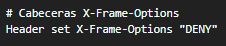
\includegraphics[width=\textwidth]{./img/vulnerabilidades/3.5/7.1.png}
                        \caption{Cabecera X-Frame-Options}
                    \end{figure}
            \clearpage
            \subsection{Cabecera X-Permitted-Cross-Domain-Policies}
                \subsubsection{Descripción}
                    La cabecera X-Permitted-Cross-Domain-Policies permite a los propietarios del contenido controlar cómo los documentos son tratados en contextos de navegación cruzada.
                \subsubsection{Solución}
                    Para solucionar este problema, crearemos una cabecera 'X-Permitted-Cross-Domain-Policies' con el valor 'none' para que el navegador no permita que se usen características y APIs en los contenidos de una página.
                    \begin{figure}[H]
                        \centering
                        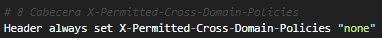
\includegraphics[width=\textwidth]{./img/vulnerabilidades/3.5/8.1.png}
                        \caption{Cabecera X-Permitted-Cross-Domain-Policies}
                    \end{figure}
            \clearpage
            \subsection{Cabecera X-DNS-Prefetch-Control}
                \subsubsection{Descripción}
                    La cabecera X-DNS-Prefetch-Control es una cabecera HTTP que se utiliza para controlar la funcionalidad de prefetching DNS en los navegadores. El prefetching DNS es una técnica que los navegadores utilizan para anticiparse a las solicitudes DNS antes de que un usuario haga click en un enlace. Esto puede acelerar la carga de páginas al preresolver los nombres de dominio antes de que se soliciten explícitamente.
                    Esto puede provocar que el navegador realice peticiones a dominios que no son de confianza, dar informacion de dominios sensibles, etc.
                \subsubsection{Solución}
                    Para solucionar este problema, crearemos una cabecera 'X-DNS-Prefetch-Control' con el valor 'off' para que el navegador no permita que se precarge contenido de la página.
                    \begin{figure}[H]
                        \centering
                        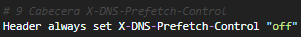
\includegraphics[width=\textwidth]{./img/vulnerabilidades/3.5/9.1.png}
                        \caption{Cabecera X-DNS-Prefetch-Control}
                    \end{figure}
            \clearpage
            \subsection{Cabecera X-Download-Options}
                \subsubsection{Descripción}
                    La cabecera X-Download-Options es una cabecera HTTP que se utiliza para controlar cómo ciertos navegadores manejan la descarga de archivos. Esta cabecera tiene un propósito específico en el contexto de Internet Explorer (IE) y se utiliza para mitigar el riesgo de ejecución automática de archivos descargados que podrían ser maliciosos.
                \subsubsection{Solución}
                    Para solucionar este problema, crearemos una cabecera 'X-Download-Options' con el valor 'noopen' para que el navegador no permita que se ejecuten los archivos descargados.
                    \begin{figure}[H]
                        \centering
                        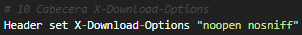
\includegraphics[width=\textwidth]{./img/vulnerabilidades/3.5/10.1.png}
                        \caption{Cabecera X-Download-Options}
                    \end{figure}
            \clearpage
            \subsection{Cabecera Referrer-Policy}
                \subsubsection{Descripción}
                    Esta cabecera controla cómo se incluye el encabezado Referer en las solicitudes. Puedes configurarlo para reducir la cantidad de información sensible enviada en las solicitudes de referencia.
                \subsubsection{Solución}
                    Para solucionar este problema, crearemos una cabecera 'Referrer-Policy' con el valor 'no-referrer' para que el navegador no envíe información sensible en las solicitudes de referencia.
                    \begin{figure}[H]
                        \centering
                        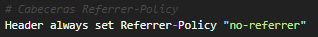
\includegraphics[width=\textwidth]{./img/vulnerabilidades/3.5/11.1.png}
                        \caption{Cabecera Referrer-Policy}
                    \end{figure}
            \clearpage
            \subsection{Cabecera Feature-Policy}
                \subsubsection{Descripción}
                    La cabecera 'Feature-Policy' permite que un sitio controle qué características y APIs pueden ser utilizadas por los contenidos de una página.
                \subsubsection{Solución}
                    Para solucionar este problema, crearemos una cabecera 'Feature-Policy' con el valor 'none' para que el navegador no permita que se usen características y APIs en los contenidos de una página.
                    \begin{figure}[H]
                        \centering
                        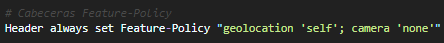
\includegraphics[width=\textwidth]{./img/vulnerabilidades/3.5/12.1.png}
                        \caption{Cabecera Feature-Policy}
                    \end{figure}
            \clearpage
            \subsection{Cabecera Expect-CT}
                \subsubsection{Descripción}
                    Las cabeceras 'Expect-CT' ayuda a proteger al usuario contra ataques de certificate transparency.
                \subsubsection{Solución}
                    Para solucionar este problema, crearemos una cabecera 'Expect-CT' con el valor 'max-age=86400' para que el navegador no permita que se usen características y APIs en los contenidos de una página.
                    \begin{figure}[H]
                        \centering
                        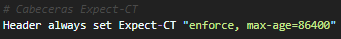
\includegraphics[width=\textwidth]{./img/vulnerabilidades/3.5/13.1.png}
                        \caption{Cabecera Expect-CT}
                    \end{figure}
            \clearpage
            \subsection{Configuración PHP}
                \subsubsection{Descripción}
                    Cuando usamos PHP en un servidor web, es importante configurarlo de forma segura para evitar que se filtre información que pueda ayudar a los atacantes a encontrar una vulnerabilidad en nuestro sistema.
                \subsubsection{Solución}
                    Hemos ocultado la versión de PHP en las peticiones a nuestro servidor para evitar que un atacante pueda usar esta información para encontrar una vulnerabilidad en nuestro sistema. Para ello, hemos creado el php.ini
                    \begin{figure}[H]
                        \centering
                        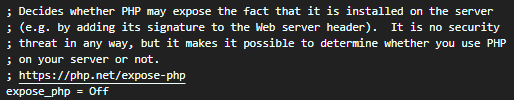
\includegraphics[width=\textwidth]{./img/vulnerabilidades/3.5/14.1.png}
                        \caption{Ocultar versión de PHP}
                    \end{figure}
            \clearpage
            \subsection{Configuración Apache}
                \subsubsection{Descripción}
                    Al igual que con PHP en el punto anterior, es importante configurar Apache para que muestre la mínima información al exterior.
                \subsubsection{Solución}
                    Para ello, al igual que con PHP, hemos ocultado las versiones del servidor para evitar en la medida de lo posible que el atacante encuentre vulnerabilidad en nuestro servidor. Para ello, hemos editado el apache2.conf
                    \begin{figure}[H]
                        \centering
                        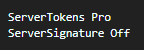
\includegraphics[width=\textwidth]{./img/vulnerabilidades/3.5/15.1.png}
                        \caption{Ocultar versión de Apache}
                    \end{figure}
            \clearpage
        \section{Componentes vulnerables y obsoletos}
            Se refiere a partes o elementos dentro de un sistema, software o hardware, que presentan vulnerabilidades de seguridad debido a su antigüedad o a la falta de actualizaciones.
            \subsection{Control de versiones de los componentes}
                \subsubsection{Descripción}
                    Es crítico mantener actualizados los sistemas operativos y el software de seguridad con las últimas actualizaciones y parches de seguridad.
                \subsubsection{Solución}
                    Para solucionar este problema, hemos actualizado todos los componentes a sus últimas versiones.
                    \begin{itemize}
                        \item PHP 7.2.2 → 8.2
                        \item MariaDB 10.8.2 → 11.1.2
                        \item phpMyAdmin 5.1.1 → 5.1.1
                        \item jQuery 3.6.0 → 3.7.1
                    \end{itemize}
                    En estos casos, es recomendable no usar latest ya que en el pasado ha sido un problema de seguridad. Esto se debe a que un atacante puede tener acceso a la imagen y alterándola provoca que todo el que use latest se descargue la versión infectada.
            \clearpage
        \section{Fallos de identificación y autenticación}
            Los fallos de identificación y autenticación se refieren a deficiencias o problemas en los procesos y mecanismos diseñados para verificar la identidad de un usuario y asegurar que la persona o entidad que intenta acceder a un sistema o recurso es realmente quien afirma ser. 
            \subsection{Captcha}
                \subsubsection{Descripción}
                    Un captcha es un tipo de prueba de Turing que se utiliza para determinar si el usuario es o no humano. Los captchas se utilizan para prevenir ataques de tipo bot, como el spam y el abuso de servicios web.
                \subsubsection{Solución}
                    Para solucionar este problema, hemos añadido un captcha a nuestro formulario de registro e inicio de sesión.
                    Hemos añadido para nuestro proyecto el reCAPTCHA v3 de Google ya que es el más fácil de implementar y el que menos molesta al usuario.
                    La puntuación se basa en las interacciones con su sitio y le permite tomar las medidas adecuadas para su sitio.
                    Es por esto que, ha diferencia de otros captchas, este no muestra ninguna imagen al usuario pero si que se ejecuta en segundo plano y, si detecta que el usuario es un bot, se le bloquea el acceso.
                    \\\\
                    \textbf{Nota:} reCAPTCHA v3 utiliza un sistema de puntuaciones que gestiona la propia Google. Esto puede hacer que al conectarte desde una VPN o una red pública te bloqueé el acceso. Ten esto en cuenta si estás accediendo desde la red de la universidad.
            \clearpage
            \subsection{Contraseñas débiles o por defecto}
                \subsubsection{Descripción}
                    Las contraseñas débiles o por defecto son contraseñas que son fáciles de adivinar o que se utilizan en muchos sistemas diferentes. Esto puede permitir a un atacante obtener acceso no autorizado a un sistema o aplicación.
                \subsubsection{Solución}
                    Para solucionar este problema, hemos hecho dos cosas:
                    \begin{itemize}
                        \item Añadir un JS que asegura que las contraseñas de nuestros usuarios cumplen con los requisitos mínimos de seguridad.
                        \begin{figure}[H]
                            \centering
                            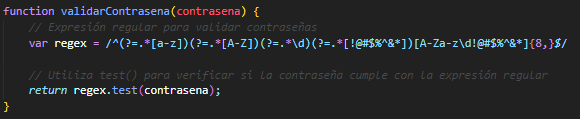
\includegraphics[width=\textwidth]{./img/vulnerabilidades/3.7/2.1.png}
                            \caption{JS de validación de contraseñas}
                        \end{figure}
                        \item Cambiar las contraseñas de nuestros servicios como phpMyAdmin, MariaDB, etc.
                        \begin{figure}[H]
                            \centering
                            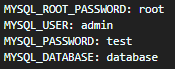
\includegraphics[width=\textwidth]{./img/vulnerabilidades/3.7/2.2.png}
                            \caption{Contraseña antes del cambio}                            
                        \end{figure}
                        \begin{itemize}
                            \item Estas contraseñas se ven dentro del .env el cual no se debería subir, pero al ser un trabajo se ha subido al repositorio.
                        \end{itemize}
                    \end{itemize}
            \clearpage
            \subsection{Invalidación de sesiones}
                    \subsubsection{Descripción}
                        La invalidación de sesiones se refiere a la práctica de terminar una sesión de usuario cuando el usuario sale de una aplicación o sitio web. Esto puede ayudar a prevenir ataques de tipo secuestro de sesión, en los que un atacante puede tomar el control de una sesión de usuario activa.
                    \subsubsection{Solución}
                        En este punto, también hemos puesto dos soluciones al problema:
                        \begin{enumerate}
                            \item Hemos añadido un botón de cerrar sesión en la página de perfil de usuario.
                            \item La cookie se cierra automáticamente al cerrar el navegador.
                        \end{enumerate}
                        Con estas dos soluciones, si un usuario se olvida de cerrar sesión, el sistema lo hará automáticamente y, si un atacante consigue la sesión de un usuario, esta se invalidará de igual forma.
            \clearpage
        \section{Fallos en la integridad de datos y software}
            Los fallos en la integridad de datos y software pueden tener graves consecuencias en la seguridad y confiabilidad de sistemas y aplicaciones. Estos fallos pueden ocurrir debido a diversas razones, y es importante abordarlos adecuadamente para mantener la integridad de los datos y el funcionamiento del software.
            \subsection{Copias de seguridad}
                \subsubsection{Descripción}
                    Las copias de seguridad son una medida de seguridad que permite a los usuarios y administradores de sistemas restaurar datos y sistemas a un estado anterior en caso de que se produzca una pérdida de datos o un fallo del sistema. Las copias de seguridad pueden ser útiles para recuperar datos perdidos debido a errores humanos, ataques de malware, fallos de hardware, desastres naturales, etc.
                \subsubsection{Solución}
                    Para solucionar este problema, debemos realizar una copia de seguridad de nuestra base de datos cada cierto periodo de tiempo.
                    En nuestro caso, accederemos a la base de datos mediante el phpMyAdmin y exportaremos la base de datos en un archivo .sql
            \clearpage
            \subsection{CI/CD}
                \subsubsection{Descripción}
                    CI/CD es un conjunto de prácticas y herramientas que permiten a los equipos de desarrollo de software entregar cambios de código de forma rápida y fiable. CI/CD es un acrónimo de Integración Continua (CI) y Despliegue Continua (CD). CI/CD es una práctica fundamental para DevOps.
                \subsubsection{Solución}
                    Para solucionar este problema, podemos generar un pipeline de CI/CD en GitHub Actions mediante los Workflows.
                    \begin{figure}[H]
                        \centering
                        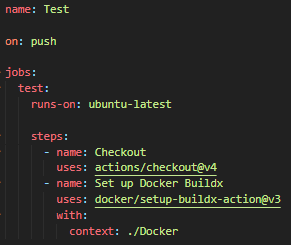
\includegraphics[width=\textwidth]{./img/vulnerabilidades/3.8/2.1.png}
                        \caption{Pipeline de CI/CD}
                    \end{figure}
                    Este no es un pipeline completo con todas las pruebas unitarias ni la creación de las imágenes ni una despliegue como el que podría ser Kubernetes, pero sirve como ejemplo para este trabajo.
            \clearpage
        \section{Fallos en la monitorización de la seguridad}
            Los fallos en la monitorización de la seguridad se refieren a deficiencias o problemas en los sistemas y procesos diseñados para vigilar y evaluar la seguridad de una red, sistema informático, aplicación o entorno en general.
            \subsection{Auditorías de seguridad}
                \subsubsection{Descripción}
                    Una auditoría de seguridad es un proceso sistemático de evaluación y revisión de sistemas, redes, aplicaciones o entornos tecnológicos con el propósito de identificar vulnerabilidades, debilidades y riesgos de seguridad. El objetivo principal de una auditoría de seguridad es garantizar que los controles de seguridad estén implementados adecuadamente y cumplan con los estándares de seguridad, y proporcionar recomendaciones para mejorar la protección de activos y datos contra amenazas y ataques cibernéticos.
                \subsubsection{Solución}
                    La solucion a este problema, es realizar un plan de seguridad para nuestro sistema y realizar auditorías de seguridad cada cierto tiempo para comprobar que no se han introducido nuevos problemas de seguridad.
            \clearpage
            \subsection{Configuración de logs del sistema}
                \subsubsection{Descripción}
                    Los logs del sistema son una herramienta de seguridad que permite a los administradores de sistemas y a los equipos de seguridad supervisar y analizar la actividad de los sistemas y las redes. Los logs del sistema pueden utilizarse para detectar y analizar incidentes de seguridad, así como para identificar y prevenir posibles amenazas.
                \subsubsection{Solución}
                    Para solucionar este problema, hemos implementado una lógica del log del lado del servidor para guardar los logs de los usuarios al cometer errores.
                    \begin{figure}[H]
                        \centering
                        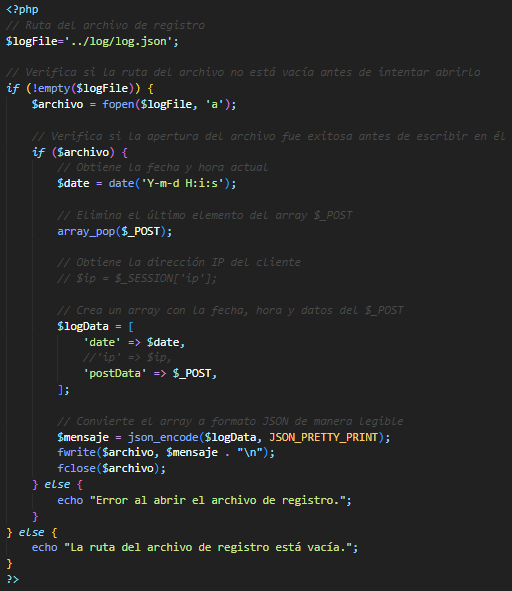
\includegraphics[width=0.9\textwidth]{./img/vulnerabilidades/3.9/2.2.png}
                        \caption{Logs del lado del servidor}
                    \end{figure}
            \clearpage
    \chapter{Segunda auditoría}
        Tras arreglar los problemas de la primera auditoría, hemos vuelto a realizar una auditoría de seguridad para comprobar que no se han introducido nuevos problemas de seguridad.
        \section{ZAP}
            Para llevar la misma estructura que en la primera auditoría, hemos usado la misma herramienta para realizar la segunda.
            \begin{figure}[H]
                \centering
                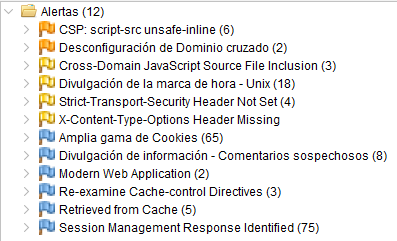
\includegraphics[width=0.8\textwidth]{./img/audit2/zap1.png}
                \caption{Listado de errores de ZAP de la segunda auditoría}
            \end{figure}
            Aunque veamos que todavia hay errores, estos en realidad son dados porque ZAP no puede comprobar algunas de las librerías que usamos en nuestro proyecto como son jQuery y reCAPTCHA.
            
            Aun así, ambas librerías hacen que nuestra web sea mas segura por lo que no las vamos a eliminar de nuestro proyecto solo para que ZAP no de errores.
        \clearpage
        \section{sqlmap}
            Para comprobar que los problemas de inyección SQL estan solucionados, hemos usado sqlmap.
            \begin{figure}[H]
                \centering
                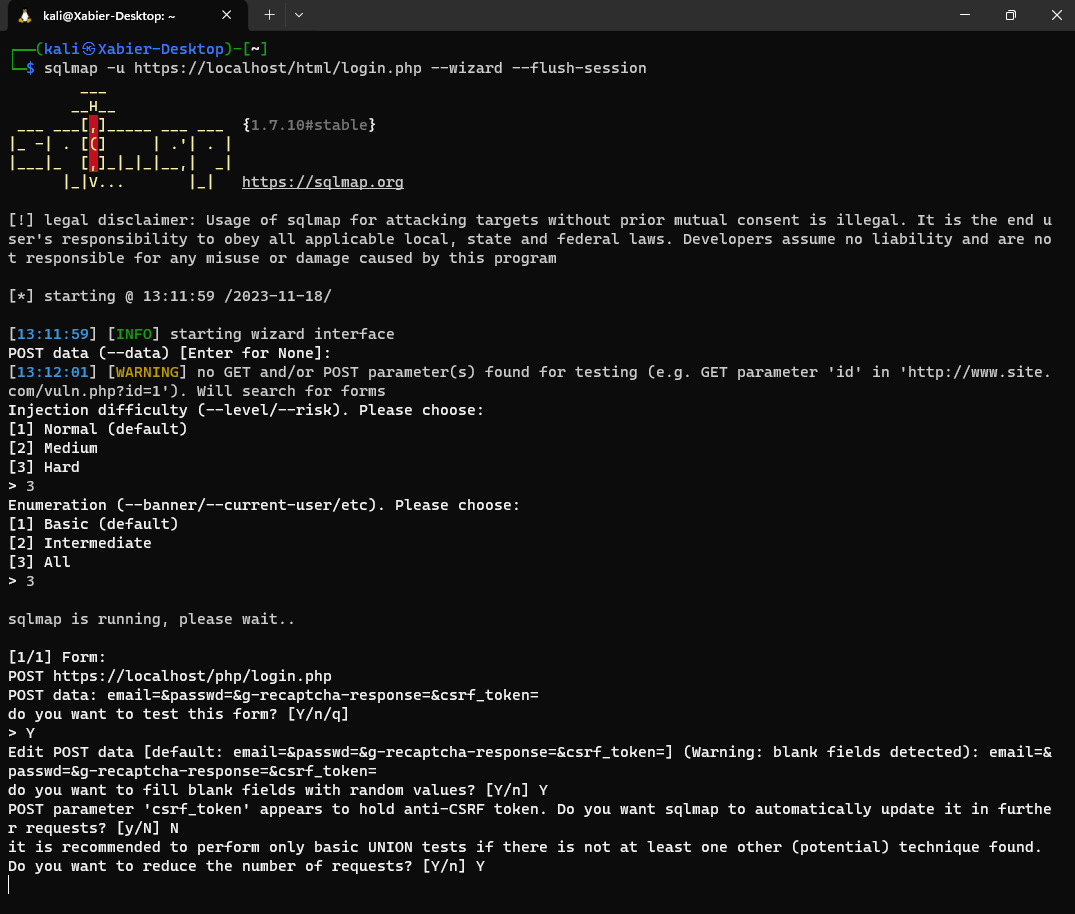
\includegraphics[width=\textwidth]{./img/audit2/sqlmap1.png}
                \caption{Output de sqlmap}
            \end{figure}
            Como podemos ver, sqlmap no ha encontrado ninguna vulnerabilidad en nuestro sistema gracias al token csrf que está impidiendo que se tramiten las peticiones maliciosas al servidor.
            \clearpage
            \begin{figure}[H]
                \centering
                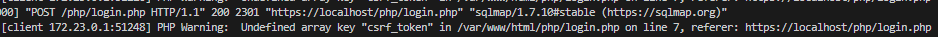
\includegraphics[width=\textwidth]{./img/audit2/sqlmap2.png}
                \caption{Logs del servidor}
            \end{figure}
            Esto se debe a que nuestra página web está pensada para cargar el contenido dinámicamente mediante AJAX y no mediante peticiones GET o POST.
            Por lo tanto, al no acceder antes al index.php, no se crea la sesión en el navegador con los tokens reCAPTCHA, CSRF y la cookie de sesión.
            Esto hace que sqlmap no pueda acceder a las páginas que requieren autenticación y, por lo tanto, no pueda comprobar si hay vulnerabilidades.
        \clearpage
        \section{nmap}
            Para comprobar que nuestro servidor web ya no aporta información sensible, hemos usado nmap.
            \begin{figure}[H]
                \centering
                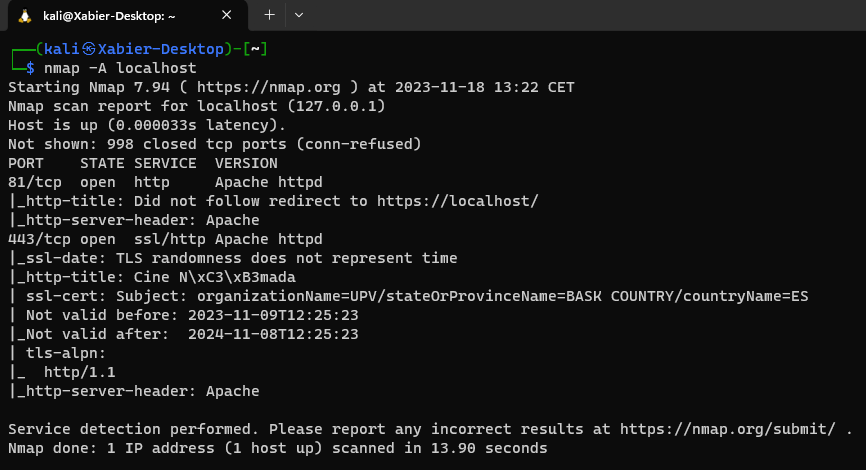
\includegraphics[width=\textwidth]{./img/audit2/nmap1.png}
                \caption{Output de nmap}
            \end{figure}
            Como podemos ver, nmap ha dejado de devolvernos información sensible como la versión de PHP o Apache y ahora nos informa de que el servidor hace una redirección al 443 con certificado SSL.
        \clearpage
        \section{Metaexploit}
            Por último, vamos a comprobar que nuestro servidor web ya no es vulnerable a ataques de fuerza bruta.
            \begin{figure}[H]
                \centering
                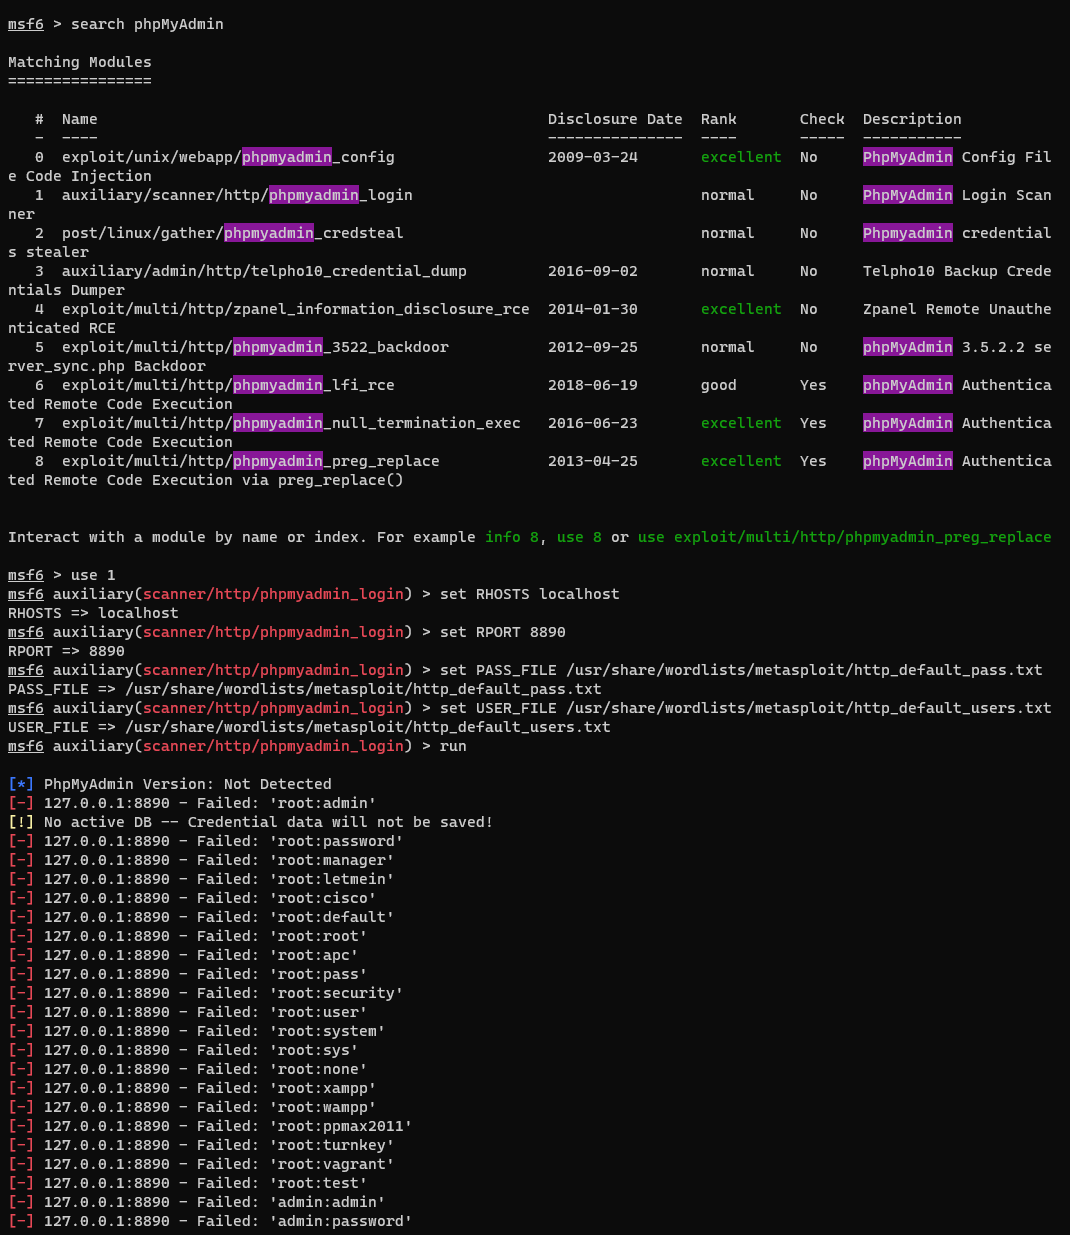
\includegraphics[width=0.9\textwidth]{./img/audit2/msf1.png}
                \caption{Output de metasploit}
            \end{figure}
            Dado que hemos cambiado las contraseñas de nuestros servicios, metasploit ya no puede acceder a ellos.
            Esta no es la mejor solución, ya que teóricamente phpMyAdmin sigue siendo vulnerable a ataques de fuerza bruta, pero dado que phpMyAdmin solo es accesible desde localhost, no es un problema de seguridad.
            Lo mismo occure con la base de datos MariaDB la cual solo es accesible mediante la web y no desde el exterior.
        \clearpage
    \chapter{Conclusiones}
        Este proyecto ha constituido una valiosa oportunidad para constatar la vulnerabilidad intrínseca de las páginas web y servicios en línea cuando no se configuran adecuadamente. La experiencia adquirida ha demostrado ser esencial, destacando la necesidad crítica de abordar las deficiencias de seguridad que pueden comprometer la integridad y confidencialidad de los datos. En el transcurso de este proceso, hemos puesto a prueba no solo nuestras habilidades de programación, sino también nuestras capacidades de investigación, al enfrentarnos a la tarea de identificar no solo las vulnerabilidades en sí, sino de concebir métodos efectivos para su mitigación y resolución.\\
        
        La comparativa entre las pruebas de penetración realizadas y presentadas en este informe revela una transformación significativa en la seguridad de la plataforma. Los ataques previamente exitosos, que tradicionalmente se emplean contra las páginas web, han perdido su eficacia. Este resultado tangible subraya el éxito de nuestras estrategias de fortificación, evidenciando el impacto positivo de las medidas implementadas. La labor llevada a cabo no solo ha consistido en cerrar brechas de seguridad, sino también en desarrollar un entorno digital robusto y resistente, capaz de hacer frente los desafíos cada vez más sofisticados que plantea el panorama actual de amenazas cibernéticas. Este proyecto, en última instancia, ha fortalecido nuestra comprensión integral de la seguridad web y ha ampliado nuestras habilidades prácticas y teóricas en este campo de estudio crucial.\\
    \chapter{Bibliografía}
        \begin{itemize}
            \item OWASP. (2021). Informe de Vulnerabilidades. OWASP. \url{https://owasp.org/www-project-top-ten/}
            \item GPT-3.5. (2023). Respuestas a preguntas varias. OpenAI. \url{https://www.openai.com/}
            \item GitHub Copilot. (2022). Autocompletado. GitHub. \url{https://github.com/features/copilot}
            \item PHP. (2021). Manual de PHP. PHP. \url{https://www.php.net/manual/es/}
            \item reCAPTCHA. (2018). Documentación de reCAPTCHA. Google. \url{https://developers.google.com/recaptcha/docs/v3}
            \item sqlmap. (2017). Documentación de sqlmap. sqlmap. \url{https://github.com/sqlmapproject/sqlmap/wiki/}
            \item ZAP. (2023). Documentación de ZAP. OWASP. \url{https://www.zaproxy.org/docs/}
            \item metasploit. (2023). Documentación de metasploit. Rapid7. \url{https://docs.rapid7.com/metasploit/}
            \item nmap. (2020). Documentación de nmap. nmap. \url{https://nmap.org/man/es/}
        \end{itemize}
\end{document}